\chapter{Stand der Technik}

Wie schon in der Einleitung erwähnt ist das Gebiet des zweihändigen Umgreifen, bzw. der Bewegungsplanung dafür, weitaus weniger stark erforscht als einhändige Greifaufgaben. Man findet eine Menge Literatur zum Thema Umgreifen mit Hilfe von \glqq Pick-and-Place\grqq{} oder zum Umgreifen in einer Hand, aber nur eine Handvoll Arbeiten betrachten eine ähnliche Problemstellung wie sie hier behandelt werden soll (vgl. ~\cite{Mousavi2013Taxonomy}).\\
Im Folgenden wird zunächst ein knapper Überblick über Arbeiten gegeben, die sich nur sehr entfernt mit dem hier behandelten Thema beschäftigen. Im Anschluss wird auf vier Publikationen im Detail eingegangen, die sich unterschiedliche Schwerpunkte bei der Suche nach einer Lösung für das zweihändige Umgreifen gesetzt haben. Insbesondere die letzten beiden Ansätze~\ref{sec:Bildverabeitung} haben erkennbare Parallelen zu einigen der Methoden die in dieser Arbeit zum Einsatz kommen.

\section{Allgemeiner Überblick}

\textcolor{red}{Fehlt!, aber gibt es wirklich was nennenswertes??}

\section{Schwerpunkt Bewegungsplanung}

\paragraph{Pick-and-Place-Tasks with Two-Hand Regrasping}

Die erste genauer betrachtete Arbeit wurde nur in der Simulation entwickelt. Allerdings setzt sie einige Methoden ein, die bei späteren Arbeiten wieder aufgegriffen wurden, darum wird sie hier im Detail behandelt. Basierend auf, im Vorhinein berechneten, Roadmaps und Griffen wird eine Bewegung für eine \glqq Pick-and-Place\grqq -Aufgabe erzeugt, bei der das Objekt in der Luft von einer Hand in die andere übergeben wird. Um das zu erreichen, haben Saut u.a. im Jahr 2010 ein System~\cite{saut2010planning} entwickelt das besonders auf Hände mit vielen Freiheitsgraden, beispielsweise 4 Fingern mit jeweils 3 Freiheitsgraden und einem zusätzlichen Daumen, spezialisiert ist.
\\

Das System ist unterteilt in einen Greif-Planer und einen Pfad-Planer. Prinzipiell kann ersteres durch einen beliebigen anderen Algorithmus der stabile, kraft-geschlossene Griffe erzeugt, ersetzt werden, aber der Vollständigkeit halber wird er hier kurz beschrieben. Ein Griff ist in diesem Fall definiert durch einen \glqq Frame\grqq{}, was die relative Pose der Hand zum Objekt beschreibt, einer Menge an Kontaktpunkten der Finger mit der Objektoberfläche und der Handkonfiguration bei geschlossenem Hand. Zuerst wird durch zufälliges Positionieren der Hand um das Objekt eine Menge an \glqq Frames\grqq{} erzeugt. Für jedes Element dieser Menge wird dann versucht einen kollisionsfreien Griff zu finden. Dafür wird die Oberfläche des betrachteten Objekt durch eine Punktwolke und der Arbeitsraum der Finger durch nicht-überschneidende Kugeln approximiert. Mit diesen Daten-Strukturen können nun effizient die Kontaktpunkte der Fingerspitzen am Objekt gefunden werden. Beginnend mit dem Daumen berechnet der Algorithmus für einen Finger nach dem anderen eine IK-Lösung\footnote{\glqq Inverse Kinematik\grqq{} \ref{sec:InverseKinematik}} der Fingergelenke und testet diese ob sie mit den bereits gefunden Konfigurationen der vorangehenden Finger kollidiert. Ist dies der Fall wird der aktuelle Griff sofort verworfen. Nachdem jedes \glqq Frame\grqq{} betrachtet wurde, werden für die gefundenen, garantiert kollisionsfreien, Griffe jeweils vier Bewertungen berechnet und mit manuell gesetzten Gewichtungen addiert~\cite[Abschnitt IV-A-3]{saut2010planning}. Basierend auf dem Resultat werden die Griffe nach Qualität sortiert und dann weiterverwendet. \\
Nun gilt es aus diesen Griffen mögliche zweihändige Griff-Paare zu erzeugen. Dafür werden zwei Listen, jeweils mit Griffen für die linke bzw. rechte Hand, genommen und zunächst jeder dieser Griffe auf Kollision mit der Umwelt an der Start- und Zielpose des Objekts getestet. Jene Kandidaten die nicht kollidierten werden nun paarweise analysiert: Kollidierende Paare werden ignoriert. Für die restlichen wird eine kombinierte Bewertung aus dem Minimum der beiden Qualitätswerte und dem Minimum einer Roboterkonfigurations-Bewertung, basierend darauf wie \glqq natürlich\grqq{} das Objekt in der Start- bzw. Zielpose mit einem der beiden Griffe gegriffen werden kann, bestimmt. Nachdem alle möglichen Paare analysiert wurden ist das Ergebnis eine Liste von nach Qualität sortierten Doppelgriffen, für die im Folgenden nun eine Übergabepose gefunden werden muss.
\\

Zur Bestimmung der Übergabe-Pose des Objekts wird zunächst die Position ermittelt. Dafür minimiert der Algorithmus die Bewegung der Handgelenke um ausgehend von der initialen Greifpose die Übergabe-Pose zu erreichen. Anschließend wird die gefundene Objektposition approximativ auf Kollisionen mit der Umwelt getestet. Die Orientierung hingegen wird anhand des gefundenen Doppel-Griffes bestimmt, indem die beiden einzelnen Handposen der gewählten Griffe und deren Position in Relation zum Robotertorso berücksichtigt werden. Abschließend wird die nun theoretisch optimale Objektpose erneut geprüft ob sie mit der Umwelt kollidiert und, wenn nicht, versucht eine IK-Lösung für den Roboter zu berechnen. Schlägt dies fehl, so wird basierend auf einer Gauß-Verteilung um das theoretische Optimum weiter versucht zunächst eine kollisionsfreie Objektpose und im Anschluss eine gültige Roboterkonfiguration zu finden.
\\

Um die Rechenzeit zum Planen der Bewegung zu reduzieren wird im Vorhinein eine \glqq Roadmap\grqq{} basierend auf ~\cite{gharbi2009roadmap} generiert. Dieser Algorithmus berücksichtigt zunächst aber nur die Umwelt und die Roboterposen in seiner Berechnung. Während der Ausführung muss das Ergebnis angepasst werden, damit auch wenn der Roboter das Objekt gegriffen hat es zu keiner Kollision kommt.\\
Die gesamte Aufgabe kann in drei relevante Teilaufgaben unterteilt werden, für die jeweils einzeln Anfragen an die PRM\footnote{\glqq Probabilistic Roadmap\grqq{}~\citep{kavraki1996probabilistic}} gestellt werden:
\begin{itemize}
\item Das, auf dem Tisch stehende, Objekt greifen
\item Das gegriffene Objekt und den Roboter zur Übergabepose bewegen (Am Ende dieser Bewegung haben beide Hände das Objekt in der Luft gegriffen)
\item Das Objekt zur Zielpose bewegen
\end{itemize}
Diese Teilbewegungen sind bei so gut wie jeder Umgreif-Aufgabe zu finden, darum werden sie hier explizit erwähnt.\\
Für jede dieser Anfragen versucht die PRM einen Pfad zu finden. Hat sie einen gefunden, so wird das Objekt in der Hand des Robotermodels entsprechend des ersten Griffes in den Arbeitsraum hinzugefügt und getestet, ob der gefundene Pfad noch immer kollisionsfrei ist. Wenn nicht, dann wird durch einen klassischen Bewegungsplaner, der bspw. auf RRTs\footnote{\glqq Rapidly-exploring random tree\grqq{}~\citep{lavalle2000rapidly} und vgl. \ref{sec:Bewegungsplanung}} basiert, versucht eine kollisionsfreie Trajektorie zu finden.
\\

Getestet wurde das System in der Simulation am humanoiden Roboter Justin~\citep{ott2006humanoid}, der mit seinen zwei feinmotorischen Händen auf insgesamt 43 Freiheitsgrade kommt. Als Testobjekt wurde eine komplexe Pferdefigur verwendet, die auch bei anderen Forschungsgruppen weit verbreitet ist. Somit sind die Ergebnisse einfach mit anderen Projekten zu vergleichen. Trotz der hohen Dimensionalität sowohl des Roboters als auch des Objekts benötigte der Planer im Schnitt nur um die 11 Sekunden um die gesamte Bewegung zu berechnen. Die vorbereitete Roadmap mit ca. 1700 Knoten konnte in 5 Minuten erzeugt werden und die beiden Griff-Listen in jeweils ungefähr einer Minute. In sehr wenigen Fällen konnte keine Lösung gefunden werden. Dies ist darauf zurückzuführen, dass bereits die Startpose des Objekts die Anzahl der kollisionsfreien Griffe soweit einschränkt, dass kein gültiges Doppel-Griff-Paar gefunden werden kann.\\
Insgesamt liefert das System sehr gute Ergebnisse, aber dadurch, dass es erwartet, dass das Objekt nach dem Greifen exakt so in der Hand liegt wie der Griff definiert ist, ist es nicht möglich solch komplexe Objekte auch in der echten Welt zu greifen, da beispielsweise mögliche Fehler zwischen Model und echtem Roboter nicht berücksichtigt werden können.


\paragraph{A Manipulation Motion Planner for Dual-Arm Industrial Manipulator}

Im Bereich der Industrie ist die möglichst effiziente Planung von mitunter komplexen Umgreif-Aktionen entscheidender als dass der Algorithmus möglichst allgemein ist. Zum einen dadurch, dass die dort eingesetzten Greifer meist auf eine überschaubare Menge an Aufgaben spezialisiert sind (z.B. in Form von Greifern mit nur zwei Fingern zum Greifen von einfach geformten Werkstücken). Zum anderen weil zu erwarten ist, dass wenn ein Objekt gegriffen wird, es danach so in der Hand liegt wie der Griff definiert ist. Dies ist ebenso auf die einfache Geometrie der zu greifenden Objekte zurückzuführen.\\

Im Jahr 2014 haben Kensuke Harada u.a. einen Manipulations-Planer vorgestellt, der allgemein für eine gegebene Aufgabe entscheidet ob dafür ein oder zwei Greifer nötig sind und welche Umgreif-Aktionen dabei umgesetzt werden müssen.\\
Der Algorithmus erwartet (wie die meisten Planer dieser Art) folgende Eingabe-Daten:
\begin{itemize}
\item Start-Pose des Objekts
\item Ziel-Pose des Objekts
\item Menge an Griffen (definiert durch die Pose des Endeffektors im Objektkoordinatensystem und die Gelenkwinkel der Finger)
\item Modell der Umwelt (kann z.B. durch eine Tiefenbild-Kamera erzeugt werden)
\end{itemize} 

Auf Grundlage dieser Informationen wird zunächst ein sog. Manipulationsgraph aufgestellt. Dieser Graph ist in 10 Bereiche mit jeweils einer Menge an Knoten unterteilt, welche in einem Vorbereitungsschritt nach und nach erzeugt werden. Eine schematische Darstellung des Ergebnisses davon ist in Abb. ~\ref{fig:Harada_ManipulationGraph} zu sehen. Dabei ist der Manipulationsraum \textit{CS} definiert durch das kartesische Produkt der Konfigurationsräume des linken Endeffektors, des rechten Endeffektors und des Objekts und in folgende Teilräume unterteilt:
\textit{CP} ist der Bereich in \textit{CS} in dem das Objekt stabil auf einer Oberfläche der Umwelt steht. \textit{CG$_{l}$} bzw. \textit{CG$_{r}$} enthält alle Konfigurationen bei denen das Objekt stabil mit dem linken bzw. rechten Endeffektor gegriffen ist.
Für die Start-/Zielpose-Bereiche wird zuerst für jedes (Pose, Griff)-Paar bestimmt ob eine kollisionsfreie IK-Lösung exisitiert. Wenn das der Fall ist, dann wird im entsprechenden Bereich ein Knoten mit der gefundenen Roboterkonfiguration hinzugefügt. Um dazwischenliegende Knoten im Bereich \textit{Intermediate object place} zu erzeugen wird für Konfigurationen bei denen das Objekt gegriffen auf einer Oberfläche steht mithilfe des \glqq Visibility\grqq -PRM-Algorithmus~\citep{simeon2000visibility} eine minimale Anzahl an Knoten in den entsprechenden Bereichen erzeugt und hinzugefügt.
Abschließend werden mögliche Übergabeposen, d.h. Konfigurationen bei denen das Objekt in der Luft von beiden Endeffektoren gegriffen ist, durch zufälliges Ausprobieren von Objekt- und Handposen gefunden.
\\
Im Anschluss werden nun Knoten aus angrenzenden Bereichen versucht miteinander durch einen Pfad zu verbinden. Je nach Pfad-Typ werden dabei unterschiedliche Strategien angewandt, die der Einfachheit halber direkt in der Arbeit \citep{harada2014manipulation} nachgelesen werden können. In jedem Fall wird jedoch der MPK-Bewegungsplaner\footnote{\url{http://ai.stanford.edu/~mitul/mpk/}} zur Berechnung verwendet.
\\

\begin{figure}[h]
\begin{center}
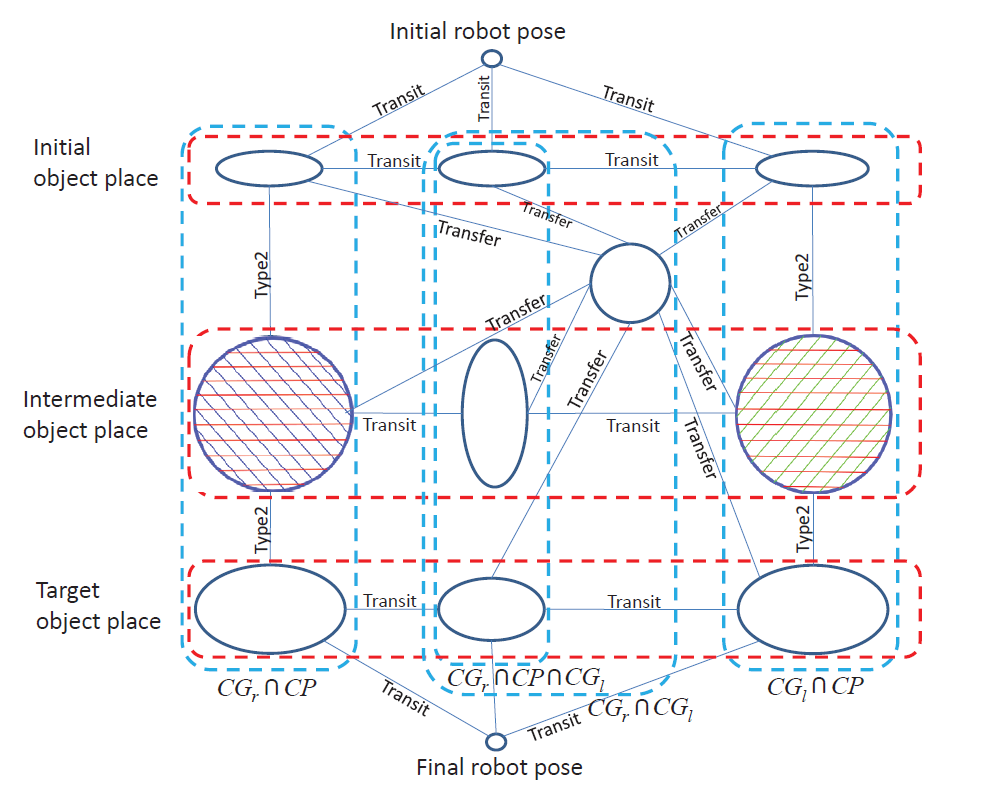
\includegraphics[width=0.7\textwidth]{Harada2014manipulation_Graph}
\caption{Generelle Struktur des Manipulationsgraphs aus~\cite{harada2014manipulation}}
\label{fig:Harada_ManipulationGraph}
\end{center}
\end{figure}

In diesem erzeugten Graph kann nun mittels Tiefensuche ein Pfad von einem Knoten im Start-Bereich zu einem Knoten im Ziel-Bereich gefunden werden. Dieser Pfad kann mitunter recht komplex werden und viele unnötige Umgreif-Bewegungen enthalten. Darum versucht im Anschluss eine vorgegebene Zeit lang ein Optimierungsalgorithmus aufeinanderfolgende Pfade zu kombinieren und zu vereinfachen. Der abschließende Pfad ist dann garantiert kollisionsfrei ausführbar. \\
Durch Verändern der Reihenfolge in der die Bereiche zuvor verbunden werden kann beeinflusst werden, ob der Roboter mit rechts oder links zugreift und ob er eher Umgreifaktionen in der Luft oder durch \glqq Pick and Place \grqq{} ausführt.
\\

Der Planer wurde am Roboter HiroNX (entwickelt von Kawada Industries Inc) getestet. Der Roboter hat zwei Arme mit jeweils 6 Freiheitsgraden und einem Industriegreifer mit zwei Fingern. Sowohl in der Simulation als auch in der echten Welt konnten Aufgabenstellungen verschiedener Schwierigkeitsstufen gelöst werden. Dabei brauchte der Planer im Schnitt zwischen 1 und 2 Minuten um eine Lösung zu finden. \\
Es existieren Videos über erfolgreiche Ergebnisse, allerdings fehlen Statistiken über die Zuverlässigkeit und Erfolgshäufigkeiten des Algorithmus. Die, zu dem Zeitpunkt, noch relativen langen Berechnungszeiten und die fehlende Berücksichtigung von möglichen ungeplanten Verschiebungen des Objekts während der Ausführung lassen einen direkten Einsatz an anderen humanoiden Robotern und mit komplexeren Gegenständen nicht ohne weiteres zu. Dennoch ist der Algorithmus in der Lage für einen beliebigen zweiarmigen idealen Roboter (ohne Fehler zwischen Model und echtem Gerät und mit exakter Ausführung) in einer beliebig komplexen Umwelt eine Lösung für ein Manipulationsproblem zu finden. Dabei wird je nach Bedarf der Aufgabenstellung eine passende Kombination aus einarmigem Greifen, zweiarmigem Greifen, Umgreifen in der Luft und Umgreifen per \glqq Pick and Place \grqq{} angewendet.


\section{Schwerpunkt Bildverarbeitung}\label{sec:Bildverabeitung}

Im Vergleich zu den beiden zuvor betrachteten Arbeiten, liegt im Folgenden der Schwerpunkt auf der Verarbeitung von Bildern des Objekts. Entweder um direkt online zweihändige Griffe bestimmten zu können, oder, wenn das Objekt bereits mit einer Hand gegriffen wurde, festzustellen, wie es in der Hand der Roboters liegt um einen gültigen Übergabegriff zu finden. Dadurch sind die beiden kommenden Systeme weniger allgemein, können dafür aber mit einer höheren Erfolgswahrscheinlichkeit auf echten Robotern angewandt werden und brauchen dabei weniger Eingaben.

\paragraph{Bimanual Regrasping from Unimanual Maschine Learning} 

Maschinelles Lernen hat sich in vielen Bereichen der Bildverarbeitung als ein mächtiges Werkzeug erwiesen. So haben auch Benjamin Balaguer und Stefano Carpin im Jahr 2010 einen Algorithmus entwickelt, der das Problem der Grifffindung sowohl auf bekannten als auch unbekannten Objekten mit Hilfe eines trainierten Systems löst. Zwei Jahre später haben sie dieses Verfahren mit einem Optimierungsalgorithmus kombiniert um stabile Umgreif-Bewegungen für beliebige Objekten generieren zu können~\citep{balaguer2012bimanual}. Nach der Trainingsphase genügt ein Stereo-Bild des auf dem Tisch stehenden Objekts als Eingabedaten.\\

Der Algorithmus besteht aus 3 Schritten (vgl. Abb. \ref{fig:Balaguer_Highlevel}):
\begin{enumerate}
\item Mit einem Merkmal-basierenden Algorithmus werden aus dem Stereo-Bildes zwei Greifpunkte auf dem Objekt bestimmt
\item Eine maschinelles Lernverfahren findet für die Greifpunkte passende Endeffektor-Orientierungen
\item Übergabepose wird durch Minimierung der benötigten Ausführungszeit der Bewegung bestimmt
\end{enumerate}

\begin{figure}[h]
\begin{center}
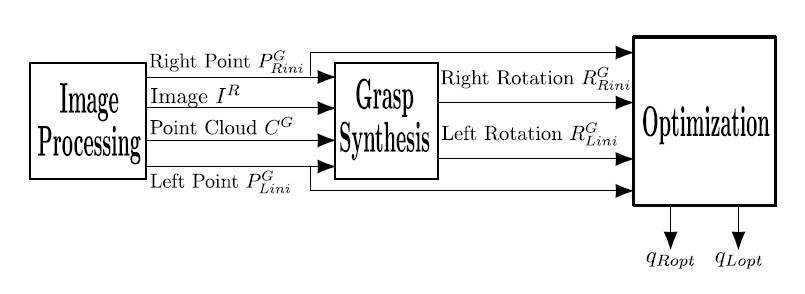
\includegraphics[width=0.7\textwidth]{Balaguer2012_Highlevel-Ablauf}
\caption{Überblick des Systems aus~\cite{balaguer2012bimanual}}
\label{fig:Balaguer_Highlevel}
\end{center}
\end{figure}

Als erster Schritt in der Bildverarbeitung wird zunächst aus dem Eingabebild die isolierte Punktwolke des Objekts erzeugt. Dafür werden alle Punkte die nicht zum Objekt gehören, d.h. beispielsweise die der Tischoberfläche, mit sog. \glqq Orthogonal Distance Regression\grqq~\citep{shakarji1998least} aus der Wolke entfernt. Danach wird das Originalbild so zurecht geschnitten, dass es auch nur noch das Objekt enthält und mit dem \glqq Canny\grqq -Algorithmus die Kanten hervorgehoben. Nur für die Pixel in der Nähe der gefundenen Kanten wird nun ein Merkmals-Vektor erstellt und mit binärer Klassifizierung entschieden ob der betrachtete Pixel ein Griffpunkt sein kann. Aus der Menge aller betrachteten Pixel werden dann zwei Punkte gewählt, die zum einen einen Abstand von mindestens 5 cm zueinander haben und zum anderen mit mindestens 90\%-iger Wahrscheinlichkeit als Griffpunkt klassifiziert werden.\\ Würde dieser Vorgang auf dem Originalbild ausgeführt werden, dann läge die Berechnungszeit bei ca. 3 Sekunden. Durch die Vorbearbeitung des Bildes und Reduzierung der Anzahl der untersuchten Pixel können die beiden Punkte in nur 130ms \citep[Abschnitt IV-A]{balaguer2012bimanual} gefunden werden, was den einen Einsatz in Echtzeitproblemstellung erlaubt.
\\

Nachdem die Griffpunkte berechnet wurden, müssen nun im Anschluss die exakten Posen der Endeffektoren gefunden werden. Die Positionen können relativ einfach durch Verschieben der Punkte orthogonal zur Objektoberfläche vom Objekt bestimmt werden, weshalb besonderes Interesse deren Orientierungen gilt. Dafür wird erneut auf maschinelles Lernen zurückgegriffen (überwachtes Lernen): Zunächst wird das Objekt als eine von \textit{N} Objektklassen identifiziert. Danach wird die Orientierung des Objekts im Bild bestimmt, indem zum einen die Ergebnisse von erneuter \glqq Orthogonal Distance Regression\grqq und zum anderen die Momente des Bildes mit vorgegebenen Trainingsdaten verglichen werden. Abschließend wird eine einfache Nächste-Nachbar-Suche in allen Trainingsdaten vorgenommen um für genau diese Griffpunkte die Endeffektor-Orientierungen zu bestimmen. Dieser Vorgang funktioniert für bekannte Objekte in 81\% der Fälle und für unbekannte Objekte immer noch in 76\% aller Fälle, was diese sog. \glqq Griff Synthese\grqq{} sehr vielseitig einsetzbar macht. Nachdem das System einmal gut eingelernt ist, muss es für neue Objekte nicht weiter angepasst werden.
\\

Im letzten Schritt wird mit den nun bekannten Posen der Endeffektoren eine Übergabe-Pose des gesamten Roboters bestimmt. Dabei wird versucht die Gelenkbewegungen und somit effektiv die Ausführungszeit zu minimieren. Die Schwierigkeit bei vielen Optimierungs-Algorithmen ist die Tatsache, dass eine Ziel-Funktion und insbesondere deren Ableitung benötigt wird. Nicht für jede Funktion lässt sich ohne weiteres ihre Ableitung bestimmen. Um dieses Problem zu umgehen basiert das hier betrachtete System auf dem \glqq Nelder-Maed\grqq -Algorithmus~\citep{nelder1965simplex}, der nur eine Kostenfunktion erwartet und zudem effizient ein Ergebnis berechnet. Für jede Objektklasse gibt es in den Trainingsdaten eine Menge an manuell bestimmten beispielhaften Übergabeposen relativ zur Roboterbasis. Aus dieser Menge werden Elemente genommen und um diese Posen herum versucht die nötigen Gelenkbewegungen zu minimieren. Die Suche nach dem Optimum findet dabei in einem 6-dimensionalen Gitter (3 Dimensionen für die Position und 3 Dimensionen für die Orientierung) in der Schnittmenge der beiden Erreichbarkeitsräumen der Endeffektoren statt. Genauere Details zu diesem Vorgang können in der Arbeit nachgelesen werden \citep{balaguer2012bimanual}.
\\

Die Arbeit behandelt nur das Bestimmen der Griffe und der Übergabepose. Für die Berechnung der Bewegung kann nun ein beliebiger Bewegungsplaner verwendet werden. Generell ist anzumerken, dass alle 3 Komponenten des Systems prinzipiell durch andere Algorithmen ersetzt werden können, somit bleibt Raum für weitere Verbesserungen und potentielle Zeiteinsparungen. Mit den hier verwendeten Teilsystemen liegt die Gesamt-Berechnungszeit auf einem Standardprozessor (2,6 GHz) bei unter 700 ms, was niedrig genug ist um an echten Robotern ohne spürbare Verzögerungen in Echtzeit Ergebnisse liefern zu können. Während der Evaluation wurden zunächst verschiedene andere Ansätze für den dritten Schritt (\glqq Optimierung\grqq) mit dem hier verwendeten Algorithmus verglichen und in allen betrachteten Aspekten (Griffqualität und Berechnungszeit) war dieser neue Ansatz besser als seine Kontrahenten. Im Anschluss wurde das gesamte System auf einem Roboter mit 22 Freiheitsgraden in der echten Welt getestet. Zuerst wurden die Griffposen vorgegeben und somit lediglich die Optimierungskomponente getestet. Dabei gelang es in 87,5\% der Fälle die Umgreif-Bewegung erfolgreich durchzuführen. Fehlschläge entstanden hierbei lediglich durch Positionsfehler des Endeffektors. Danach wurden alle Schritte von der Bildverarbeitung bis zur Bewegungsausführung getestet und in 75\% der Fälle war dies erfolgreich. Die größte Fehlerquelle hierbei war die Tatsache dass keine gute Orientierung für die Posen der Endeffektoren gefunden werden konnten. 


\paragraph{A Novel Pipeline for Bimanual Handover Tasks}

Um dieses Kapitel abzuschließen folgt nun noch eine Zusammenfassung eine kürzlich veröffentlichen Arbeit zum zweihändigen Umgreifen, die, ebenso wie das System das in dieser Arbeit entwickelt wurde, nicht darauf angewiesen ist, dass das Objekt nach dem Greifen genauso in der Hand liegt wie der Griff definiert ist, sondern direkt die relative Objektpose in der Hand bestimmt und auf Grundlage dieser Information die weiteren Bewegungen plant. Durch diese Verallgemeinerung können die Umgreif-Bewegungen zuverlässiger in der echten Welt ausgeführt werden, da mögliche Ungenauigkeiten bei der Positionierung der Endeffektoren ausgeglichen werden können. Mit diesem Hintergedanken haben Vezzani u.a. 2017 eine effiziente Pipeline (siehe Abb. \ref{fig:Vezzani_Highlevel} entwickelt~\citep{vezzani2017novel}, die einige Methoden einsetzt wie sie auch hier verwendet werden. Darum ist der Ansatz interessant um Vergleiche zu ziehen.

\begin{figure}[h]
\begin{center}
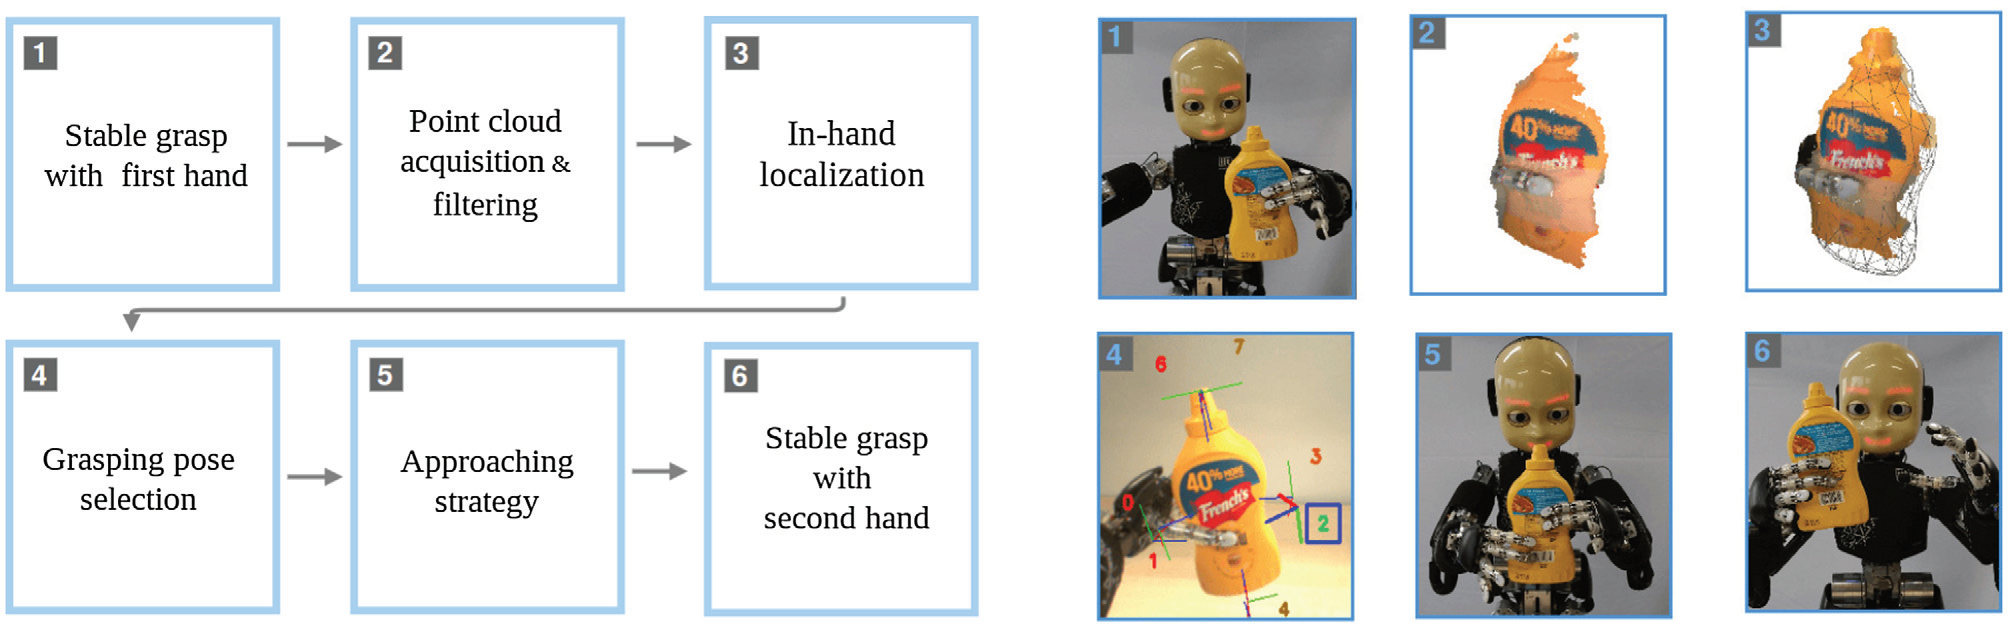
\includegraphics[width=\textwidth]{Vezzani2017_Ablauf}
\caption{Links: Ablauf der Pipeline aus~\cite{vezzani2017novel}, Rechts: Momentaufnahmen der Ausführung am echten Roboter~\citep{metta2010icub}}
\label{fig:Vezzani_Highlevel}
\end{center}
\end{figure}

Ausgehend von der Annahme, dass der Roboter das Objekt bereits auf beliebige Art und Weise gegriffen hat, zusammen mit dem Objektmodel und einer Menge an vorberechneten Griffen für das Objekt als Eingabedaten wird zunächst mithilfe von visuellen Sensoren die Objektpose in der Hand bestimmt. Dafür wird aus einem Stereo-Bild die korrespondierende Punktwolke erzeugt. Aus dieser Wolke werden dann die Ausreißer entfernt und mittels eines Farbfilters alle Punkte die zum Roboter gehören herausgenommen. Danach enthält die Wolke nur noch Punkte der Objektoberfläche Es wird hier deutlich, dass der Algorithmus nur mit Objekten funktionieren kann, die nicht grau/schwarz sind, da das die gängigen Farben von mechanischen Bauteilen oder der Verkleidung von Robotern sind. Theoretisch ist es möglich über die Vorwärts-Kinematik\ref{sec:InverseKinematik} die Pose der Hand zu bestimmen, und damit die unerwünschten Pixel zu identifizieren. Allerdings ist dieses Verfahren für Roboter die Kabelzüge (so wie der hier verwendete) oder andere mechanische Komponenten, die zum Beispiel durch Alterung ihre Eigenschaften verändern, haben nicht einsetzbar, da die Vorwärts-Kinematik unter Umständen falsche Posen berechnet. \\
Mit der gefilterten Punktwolke wird nun mit Hilfe eines angepassten \glqq Memory Unscented Particle Filter\grqq{} (MUPF) ~\citep{vezzani2017memory} die Pose des Objekts bestimmt. Der Filter-Algorithmus erwartet ein stabiles Objekt was durch die integrierte Griff-Stabilisierung der Pipeline garantiert ist. Vereinfacht ausgedrückt wird dann in mehreren Iterationen versucht das bekannte Modell des Objekts möglichst gut in die Punktwolke hineinzusetzen, so dass die Unterscheide zwischen Modelloberfläche und den einzelnen Punkten möglichst gering sind. Über die Zeit wird die vermutete Pose immer exakter, bis schließlich die Wahrscheinlichkeit, dass die aktuell vermutete Pose korrekt ist, einen bestimmten Schwellenwert überschreitet. Der genaue Algorithmus ist in der Originalarbeit nachzulesen.
\\

Der nächste Schritt besteht nun darin eine Übergabe-Pose für das Objekt zu bestimmen. Dafür wird es entsprechend der relativen Pose zum greifenden Endeffektor zum Robotermodell hinzugefügt und eine gemeinsame kinematische Kette beider Arme konstruiert. Für jedes Element einer im Vorhinein berechneten Liste an möglichen Griffen für das aktuelle Objekt werden folgende Schritte ausgeführt und zu entscheiden welche Griff am besten zu Umgreifen geeignet ist:
\begin{enumerate}
\item Setzen der Wurzel der kinematischen Kette auf den Punkt, den der freie Endeffektor erreichen soll (definiert durch den aktuell betrachteten Griff)
\item Berechnen einer IK-Lösung für beide Arme mit einem nicht-linearen Optimierungsalgorithmus (ähnlich wie in dieser Arbeit, vgl. ~\ref{sec:ConstrainedIK})
\item Berechnen des Abstands zwischen den beiden Endeffektoren in der Zielkonfiguration und einer Bewertung für die Manipulierbarkeit der gefunden Roboterkonfiguration
\end{enumerate}

Schließlich wird der Griff, für den es eine kollisionsfreie IK-Lösung gibt und dabei die besten Bewertungen hat, für die Umgreif-Aktion ausgewählt. \\
Für die Umgreifbewegung muss nun lediglich der freie Endeffektor zur berechneten Pose bewegt werden, während das Objekt durch die erwähnte integrierte Griffstabilisierung stabil in seiner Pose bleibt. Diese Stabilisierung gleicht auch mögliche ungeplante Kontakte mit dem Objekt während dem Zugreifen aus. Nach die Hand gewechselt wurde wird auch im neuen Griff das Objekt stabilisiert und somit sichergestellt, dass es nicht aus der Hand fällt.
\\

Das System wurde ausgiebig am humanoiden Roboter iCub~\cite{metta2010icub} getestet. Als Testobjekte wurde, wie auch in dieser Arbeit, 5 Objekte aus der YCB-Datenbank\footnote{\glqq Yale-CMU-Berkeley Object and Model Set\grqq{}~\citep{calli2015ycb}} genommen. Mit 100 betrachteten Elementen aus der Punktwolke braucht der MUPF-Algorithmus ungefähr 45s um die Objektpose zuverlässig zu bestimmen. D.h. ohne weiterreichende Weiterentwicklung dieses Algorithmus ist die Pipeline noch nicht für Echtzeit-Anwendungen einsetzbar. Mit allen Komponenten aktiv war die Übergabe je nach Objekt in 80-100\% erfolgreich. Diese Werte sind unabhängig von der initialen Pose der Objekts. Allerdings lässt diese Quote spürbar nach, wenn die Griffstabilisierung ausgeschaltet wird. In dem Fall konnte das Objekt nur in ca. 50\% der Fälle erfolgreich übergeben werden, da hier die Objektpose in der Hand nicht genau genug bestimmt werden konnte. Besonders gut funktioniert der Algorithmus mit Box-förmigen Objekten.